\documentclass{article}
\usepackage[margin=1.25in]{geometry}
\usepackage{graphicx}
\usepackage{titlesec}
\usepackage{geometry}
\usepackage{amsmath}
\usepackage{hyperref}
\usepackage{array}
\usepackage{empheq}
\usepackage{amsfonts}   % math fonts
\usepackage{amssymb}    % extra math symbols
\usepackage{amsthm}
\usepackage{mathtools}
\usepackage{verbatim}   % \begin{comment} multi-line comments \end{comment}
\usepackage{color}
\usepackage{xcolor}
\DeclareMathOperator*\lowlim{\underline{lim}}
\DeclareMathOperator*\uplim{\overline{lim}}
\hypersetup{hidelinks}
\setcounter{secnumdepth}{0}      % \textcolor{red}{colorful text}
\newcommand{\tb}[1]{\textbf{#1}}
\newcommand{\al}{\alpha}
\newcommand\blfootnote[1]{%
  \begingroup
  \renewcommand\thefootnote{}\footnote{#1}%
  \addtocounter{footnote}{-1}%
  \endgroup
}
\linespread{1.7}
\title{Analysis daily problems}
\author{Maxwell Gong}
\date{Start from Jan 2024}
\geometry{left = 2.5cm, right = 2.5cm}
\begin{document}
\maketitle $\blfootnote{Made by \LaTeX}$

\newpage
% Everyday there is five problems except for some special conditions 
\tableofcontents
\newpage
\section{Day 1}
\hypertarget{target}{}
\textbf{Q1}  (Sum of Series)\\
If $\sum a_n$ and $\sum b_n$ are both convergent, conclude about $\sum (a_n + b_n) $\\
\textbf{Proof} : Because $\sum a_n $, $\sum b_n $ convergent, suppose $\sum a_n \rightarrow A$, 
$\sum b_n \rightarrow B$. By definition of convergence, we have $\forall \epsilon > 0$, $\exists N_1, N_2 \in \mathbb{N}$,
$\forall n \geq N_1$, we have 
$$
\left | \sum_{k = 1}^{n} a_k  - A \right | < \epsilon
$$
And this implies that 
$$
A - \epsilon < \sum_{k=1}^{n} a_k < A + \epsilon
$$
Similarly, we have $\forall n \geq N_2$, we have
$$
B - \epsilon < \sum_{k=1}^{n} b_k < B + \epsilon
$$
Now I claim that $\sum (a_k + b_k) \rightarrow A+B$. We can take $N = max\{N_1,N_2\}$,
hence $\forall n \geq N $, 
$$
A+B - 2\epsilon < \sum_{k=1}^{n} (a_k + b_k) = \sum_{k =1 }^{n} a_k +\sum_{k=1}^{n} b_k
< A + B + 2\epsilon
$$
Hence we can say that $\sum (a_k + b_k) \rightarrow A+B$\\
\textbf{Extended question}: What about $\sum a_k b_k$ ? \\
One can show that this can be either convergent or divergent.\\
Case 1, it is divergent:\\
Let $a_n = \frac{(-1)^n}{\sqrt{n}}$ and $b_n = a_n$. By alternating series test,
one can show that $\sum a_k b_k = \sum \frac{1}{n} $, which means that even if 
$\sum a_k$ and $\sum b_k$ are convergent, $\sum a_k b_k$ is divergent.\\
The divergent case is very obvious so we do not leave a construction here. But we notice that 
if $\{a_n\}$ and $\{b_n\}$ are all positive sequences, then $\sum a_k b_k$ must be convergent.
\\
\\
\textbf{Q2} (Sum of neighbour terms)\\
If $\sum (a_n + a_{n+1})$ is convergent. Will $\sum a_n$ be convergent ?\\
\textbf{Answer}: No, we can actually give counterexample for this. Just let $a_n = (-1)^n$,
then we have $a_n + a_{n+1} = 0$. So $\sum (a_n + a_{n+1})$ is convergent.
However, if $\{a_n\}$ is positive sequence, then we are able to deduce that $\sum a_n$ 
must be convergent since 
$$
\sum a_n < \sum (a_n + a_{n+1}) \leq A
$$
where A denotes the limit of $\sum (a_n + a_{n+1})$. As $\sum a_n$ is bounded, it is 
convegent.
\\
\\
\\
\\
\\
\textbf{Q3} (Exchange odd and even terms)\\
Suppose $\sum a_n$ is convergent to S. If for all n, we exchange the position of
$a_{2n-1}$ and $a_{2n}$, prove that the new series 
$\sum a_n'$ is convergent, and find its sum.\\
\textbf{Proof}: Define $s_{n} = \sum_{k=1}^{n} a_k'$. We will next consider $\{s_{2n}\}$ and $\{s_{2n+1}\}$. Since $\sum_{n=1}^{\infty} a_n$ is convergent, so we have two things. One thing 
is that $\sum_{n=1}^{\infty} a_n = A$ and $\lim_{n \to \infty} a_n = 0$\\
So $\forall \epsilon > 0 $, $\exists N_1 \in \mathbb{N}$, $\forall n \geq N_1$,
$$
\left | \sum_{k=1}^{n} a_k - A \right | < \epsilon
$$
Take $N > \frac{N_1}{2}$. So we have $\forall n \geq N$, $2n \geq N_1$, hence
$$
\left | s_{2n} - A \right | = \left | \sum_{k=1}^{2n} a_k - A\right | < \epsilon
$$
Now we have $s_{2n} \rightarrow A$ as $n \rightarrow \infty$.\\
Since $\lim_{n \to \infty} a_n = 0$, $\exists N_2$, $\forall n \geq N_2$, $\left | a_n \right | < \epsilon$.
So let's take $N = max \{N_2,\frac{N1}{2}\}$, $\forall n \geq N$, we have $2n+1 \geq N_1$ and $2n \geq N_2$. So 
$$
\left | s_{2n+1} - A \right | = \left | \sum_{k=1}^{2n} a_k + a_{2n+2} - A \right | < \left | \sum_{k=1}^{2n} a_k - A \right | + \left | a_{2n+2} \right | < \epsilon + \epsilon = 2\epsilon
$$
\\
\\
\\
\\
\\
\textbf{Q4} (Can $a_n \ne 0$ ?)
Suppose we have positive sequence $\{a_n\}$. $\sum a_n$ is convergent. Suppose $s_n = \sum_{k=1}^{n} a_k, s_n \rightarrow S$ as $n \rightarrow \infty$.
Define $R_n = S - s_n$.\\
I leave this question as practice when I review analysis.\\
Prove that if $a_n \leq a_n R_n $, then $\sum a_n$ is a sum of finite terms.
\\
\\
\\
\\
\\
\subsection{Kummer test for convergence}
\textbf{Q5} (Kummer Test)\\
Prove that series of positive terms $\sum_{n=1}^{\infty}a_n$ convergent iff there exists positive sequence
$\{b_n\}$ and positive number $\delta > 0$, for big enough n, we have
$$
b_n \cdot \frac{a_n}{a_{n+1}} - b_{n+1} \geq \delta > 0
$$
\textbf{Proof}: \\
($\Longrightarrow$) Suppose $\sum_{n=1}^{\infty}a_n$ is convergent. Then define $b_n = \frac{R_n}{a_n}$, so we have
$b_n > 0$ since $a_n >0 $ and $R_n > 0$ as defined before. So, 
$$
b_n \cdot \frac{a_n}{a_{n+1}} - b_{n+1} = \frac{R_n}{a_{n+1}} - \frac{R_{n+1}}{a_{n+1}} = 1 > 0
$$
Notice that this is for all n.\\
($\Longleftarrow$) Consider we have 
$$
b_n \cdot \frac{a_n}{a_{n+1}} - b_{n+1} \geq \delta > 0
$$
for $n \geq N$, we can actually discard the previous terms in $\sum a_n $. So wlog, we assume this 
inequality holds for all $n$. Since $a_{n+1}$ is positive, so we multiply it both sides to obtain 
$$
a_n b_n - a_{n+1} b_{n+1} \geq \delta a_{n+1} > 0
$$ 
Then we sum both sides, we obtain the inequality such that 
$$
\sum_{n=1}^{N}\delta a_{n+1} \leq \sum_{n=1}^{N} (a_n b_n- a_{n+1} b_{n+1}) = a_1 b_1 - a_{N+1} b_{N+1} < a_1 b_1
$$
hence we can deduce that $\sum a_n$ is bounded above. So $\sum a_n$ is convergent. Done!
\newpage
\section{Day 2}
\subsection{Kummer test for divergence}
\textbf{Q1} (Kummer test for divergence)\\
$\sum_{n=1}^{\infty} a_n$ is divergent iff there exists divergent postive terms series 
$\sum_{n=1}^{\infty} \frac{1}{b_n}$, such that for big enough n, we have
$$
b_n \cdot \frac{a_n}{a_{n+1}} - b_{n+1} \leq 0
$$
We will come back to this proof later after we prove Sapagof test for convergence.\\
\\
\\
\\
\\
\textbf{Q2} ($\sum a_n$ and  $\sum \frac{1}{a_n}$)\\
Prove first that if $\sum a_n$ is convergent, then $\sum \frac{1}{a_n}$ is divergent, given that $a_n \ne 0$.
Notice that this is true for all series, we are not only restrict in positive terms series. Can you show that even 
if $\sum \frac{1}{a_n}$ is divergent, but $\sum{a_n}$ might not be convergent.\\
\textbf{Proof}: Suppose $\sum a_n$ is convergent, then $\lim_{n \to \infty} a_n = 0$. Now let's take $\epsilon = 1$,
by definition of the limit, $\exists N \in \mathbb{N}$, $\forall n \geq N$, we have $\left | a_n \right | < 1$. This 
implies that $\left| \frac{1}{a_n} \right| \geq 1$. So $\lim_{n \to \infty} \frac{1}{a_n} \ne 0 $. As a result, it must be divergent.\\
Consider $a_n = 1$. Both $\sum \frac{1}{a_n}$ and $\sum a_n$ are divergent.\\
\\
\\
\\
\\
\subsection{Saoagof test}
\textbf{Q3} (Sapagof test)\\
Suppose there is a positive decreasing sequence $\{a_n\}$, then $\lim\limits_{n \to \infty} a_n = 0$ iff postive terms series
$\sum_{n=1}^{\infty} (1-\frac{a_{n+1}}{a_n})$ is divergent.\\
\textbf{Proof}: \\
($\Longrightarrow$) Can we prove that $1 - \frac{a_{n+1}}{a_n}$ does not tend to 0 as $n \rightarrow \infty$? Obviously we can't do this. Since we can simply by
picking an counterexample to tell ourselves that there might be exceptional cases. For example, we can let $a_n = \frac{1}{n}$.\\
However, comparing to this test, proving whether a sequence is a Cauchy sequence is the stronges way we can use to prove whether a series is convergent.\\
Now, let 
$$
S_n = \sum_{k=1}^{n} (1-\frac{a_{k+1}}{a_k})
$$
we can see that
$$
S_{n+p} - S_n = \sum_{k=n+1}^{n+p}(1-\frac{a_{k+1}}{a_k}) > \frac{a_{n+1}-a_{n+p}}{a_{n+1}} = 1-\frac{a_{n+p}}{a_{n+1}}
$$
Notice that we can take $p$ to be large enough and since $a_n \rightarrow 0$, so we can make $\frac{a_{n+p}}{a_{n+1}}$ to be small enough. So we conclude that 
it is not a Cauchy sequence, so it does not convergent.\\
($\Longleftarrow$) We prove this side by contrapositive.\\
Suppose $\lim_{n \to \infty} a_n = a \ne 0$, then
$$
\sum (1-\frac{a_{n+1}}{a_n}) \leq \frac{\sum (a_k - a_{k+1})}{a} = \frac{a_1 - a }{a}
$$
Hence we can conclude that $\sum (1-\frac{a_{n+1}}{a_n})$ is convergent.\\
\\
\\
\\
\\
\textbf{Q4} (Other forms of Sapagof test) \\
Prove first that if $\{a_n\}$ is positive monotone increasing sequence, then $a_n$ is convergent iff $\sum (1-\frac{a_n}{a_{n+1}})$ is 
convergent.\\
Also show that if $S_n = \sum_{k=1}^{n} a_k$ for a positive terms series $\sum a_n$. Then $\sum a_n$ is convergent iff $\sum \frac{a_n}{S_n}$ is convergent.\\
\textbf{Proof}: \\
($\Longrightarrow$)Consider if $\{a_n\}$ is positive monotone increasing sequence. We have 
$$
1-\frac{a_n}{a_{n+1}} = \frac{a_{n+1}-a_{n}}{a_{n+1}} > 0 
$$
And one can use similar method to show that this series is bounded. This is because
$$
\sum (1-\frac{a_n}{a_{n+1}}) < \frac{\sum (a_{n+1}-a_n)}{a_1} = \frac{a-a_1}{a_1}
$$
Hence this series is bounded above, so it is convergent as it is a positive terms series.\\
($\Longleftarrow$)Again we use contrapositive to prove this. Suppose $\{a_n\}$ is divergent, i.e $a_n \rightarrow \infty$ as $n \rightarrow \infty$. 
Then I will prove that $\sum_{k=1}^{n} (1-\frac{a_k}{a_{k+1}})$ is not Cauchy sequence.\\
Just consider 
$$
\sum_{k=n}^{n+p} \frac{a_{k+1}-a_k}{a_{k+1}} > \frac{a_{n+p+1}-a_n}{a_{n+p+1}} = 1-\frac{a_n}{a_{n+p+1}}
$$
So that we can take p to large enough, we can always find such a p for $\sum_{k=n}^{n+p} \frac{a_{k+1}-a_k}{a_{k+1}} > \frac{1}{2}$.\\
The proof for \textbf{next one} just need us to notice that
$$
\sum \frac{a_n}{S_n} = \sum \frac{S_n-S_{n-1}}{S_n} = \sum 1 - \frac{S_{n-1}}{S_n}
$$
where $S_n$ is a monotone increasing positive sequence, it convergent iff $\sum (1-\frac{S_n}{S_{n+1}})$ is convergent by Sapagof test. So we proved such statement.\\
\\
\\
\\
\\
I will go back for Kummer test now. \\
\textbf{Proof}: \\
($\Longrightarrow$)If $\sum a_n$ is divergent, then just let $b_n = \frac{S_{n}}{a_n}$. Hence we have 
$$
\frac{S_n - S_{n+1}}{a_{n+1}} = \frac{-a_{n+1}}{a_{n+1}} = -1 < 0
$$
Hence we have this inequality for all n, this side is done.\\
($\Longleftarrow$)I will now prove that $\sum a_n$ is divergent. Wlog, let's assume the inequailty above holds for all n.
So we have 
$$
\frac{a_n}{a_{n+1}} \leq \frac{b_{n+1}}{b_{n}}
$$
It is equivalent to
$$
a_{n+1} \geq \frac{a_n b_n}{b_{n+1}} \geq \frac{b_n}{b_{n+1}} \cdot \frac{b_{n-1}}{b_n} \cdot a_{n-1}
$$
Carrying on this inequailty, we have $a_{n+1} \geq \frac{b_1\cdot a_1}{b_{n+1}}$ by induction. Hence use comparison test, we ca show that 
$\sum a_n$ is divergent.\\
\\
\\
\\
\\
\textbf{Q5} (One Putnam question)\\
Show first that if $\lim_{n \to \infty} (x_n - x_{n-2}) = 0$, then $\lim_{n \to \infty} \frac{x_n}{n} = 0$. Then given the same condition, show that
$$
\lim_{n \to \infty} \frac{x_n - x_{n-1}}{n} = 0
$$
(Just use this question as a review for sequence.)
\newpage
\section{Day 3}
\textbf{Q1} (The limit of a recursion sequence)\\
Suppose sequence $\{a_n\}$ satisfy $0<a_1<1$ and $a_{n+1} = a_n (1-a_n)$. Prove
$$
\lim_{n \to \infty} n \cdot a_n = 1
$$
\textbf{Proof}: Notice that 
$$
a_{n+1} - a_n = a_n - a_n^2 - a_n = - a_n^2 <0
$$
this means that the sequence is decreasing. Also, the sequence is bounded below by 0, which we can check by induction.
Then we can assume $\lim_{n \to \infty} a_n = a$. Take limit both sides on the recursion formula, one can verify that 
$$
a = a - a^2
$$
We solve the equation, so we get that $\lim_{n \to \infty} a_n = 0$.\\
Now consider $n \cdot a_n$, notice that $n \cdot a_n = \frac{n}{\frac{1}{a_n}}$. Additionally we can check the denominator is increasing and tends to infinity. Now 
we can apply Stolz in this limit, we get
$$
\lim_{n \to \infty} n \cdot a_n = \lim_{n \to \infty}\frac{n}{\frac{1}{a_n}}=\lim_{n \to \infty} \frac{n-(n-1)}{\frac{1}{a_n}-\frac{1}{a_{n-1}}} = \lim_{n \to \infty} \frac{a_n a_{n-1}}{a_{n-1}-a_n} = \lim_{n \to \infty} \frac{a_n}{a_{n-1}}
$$
To compute the limit $\frac{a_n}{a_{n-1}}$, we notice that $\frac{a_{n+1}}{a_n} = 1 - a_n$. Take limit both sides, we can show that $\lim_{n \to \infty} \frac{a_n}{a_{n-1}} = 1$. We use the fact that $\lim_{n \to \infty} a_n = 0$ here.\\
\\
\\
\\
\\
\textbf{Q2} (Divergent series's convergent Arithmetic mean)\\
Suppose $\{a_{2k-1}\}$ is convergent to $a$, $\{a_{2k}\}$ is convergent to $b$. Prove that 
$$
\lim_{n \to \infty} \frac{a_1 + a_2 + \dots +a_n}{n} = \frac{a+b}{2}
$$
\textbf{Proof}: Define $S_n = \frac{a_1 + a_2 + \dots + a_n}{n}$. By considering $\{S_{2n}\}$ and $\{S_{2n+1}\}$, one can get remarkable result. I'll first prove that
$S_{2n} \rightarrow \frac{a+b}{2}$ as $n \rightarrow \infty$. Notice that 
$$
S_{2n} = \frac{a_1 + a_2 + \dots + a_{2n}}{2n} = \frac{1}{2} \cdot \frac{a_1 + a_3 + \dots + a_{2n-1}}{n} + \frac{1}{2} \cdot \frac{a_2 + a_4 + \dots + a_{2n}}{n}
$$
By Stolz, 
$$
\lim_{n \to \infty} \frac{a_1 + a_3 + \dots + a_{2n-1}}{n} = \lim_{n \to \infty} \frac{a_{2n+1}}{1} = b
$$
Similarly, we can prove that $\lim_{n \to \infty} \frac{a_2 + a_4 + \dots + a_{2n}}{n} = a$. Hence we have $S_{2n} \rightarrow \frac{a+b}{2}$ as $n \rightarrow \infty$.\\
Next, I'll prove that $S_{2n+1}$ also has a limit of $\frac{a+b}{2}$. Notice
$$
S_{2n+1} = \frac{a_1 + a_2 + \dots + a_{2n+1}}{2n+1} + \frac{a_2 + a_4 + \dots + a_{2n}}{2n+1}
$$
Using Stolz again, one can show that $S_{2n+1} \rightarrow \frac{a+b}{2}$. Done!\\
\\
\\
\\
\\
\subsection{Inequailty about $e$}
\textbf{Q3} (An inequality about $n!$)\\
Prove that 
$$
\left (\frac{n+1}{e} \right )^{n} < n! < e \cdot \left (\frac{n+1}{e}\right )^{n+1}
$$
Use this to deduce the limit of
$$
\lim_{n \to \infty} \frac{n}{\sqrt[n]{n!}}
$$
\textbf{Proof}: If $n = 1$, inequailty denotes that $2< e <4$, which is obviously true. By mathematical induction, we have
$$
\left (\frac{n}{e} \right )^{n-1} < (n-1)! < e\cdot \left (\frac{n}{e} \right )^n
$$
One can show that
$$
n! = n \cdot (n-1)! > n \cdot \left( \frac{n}{e} \right) ^ {n-1} = \frac{n^n}{e^n} \cdot e > \left(\frac{n+1}{e}\right) ^n
$$
In the final inequailty, we use the fact that $e > \left(1+\frac{1}{n}\right)^n$. We are done on the left inequality, then we give insight into the right inequailty.
Notice that 
$$
n! = n \cdot (n-1)! < n \cdot e \cdot \left(\frac{n}{e}\right)^n = \frac{n^{n+1}}{e^{n+1}} \cdot e^2 < \frac{n^{n+1}}{e^{n+1}} \cdot \left(1+\frac{1}{n}\right)^{n+1} < e \cdot \left(\frac{n+1}{e}\right)^{n+1}
$$
where we use the inequality $e < \left( 1 + \frac{1}{n}\right)^{n+1}$.\\
We then use this fact to find an upper and lower bound of $\frac{n}{\sqrt[n]{n!}}$. Which is
$$
\frac{e \cdot n}{ \left ( n+1 \right ) \cdot \left(n+1\right)^{\frac{1}{n}}} < \frac{n}{\sqrt[n]{n!}} < \frac{e \cdot n}{n+1}
$$
Using sandwich's theorem, we can deduce that
$$
\lim_{n \to \infty} \frac{n}{\sqrt[n]{n!}} = e
$$\\
\\
\\
\\
\\
\textbf{Q4} If $\lim_{n \to \infty} a_n = a$ and $\lim_{n \to \infty} b_n = b$. Prove that 
$$
\lim_{n \to \infty} \frac{a_1 b_n + a_2 b_{n-1} + \dots + a_n b_1}{n} = a \cdot b
$$
I will leave this as an exercise for me to review since it includes very important method dealing with this kind of questions.\\
\\
\\
\\
\\
\textbf{Q5} (Equivalent definition for limit of function)\\
Prove the following two definition are equivalent.\\
I $\forall \epsilon > 0$, $\exists \delta = \delta(\epsilon) > 0$, $\forall x \in \mathbb{R}$, $0<\left| x - x_0 \right|<\delta \implies \left| f(x) - y \right| < \epsilon$\\
II $\forall J \subset \mathbb{R}$ containing $y$, $\exists I \subset \mathbb{R}$ containing $x_0$, such that $f\left(I \setminus \{x_0\}\right) \subset J$, where $J$ and $I$ are open intervals.\\
\textbf{Proof}:\\
(I $\Longrightarrow$ II) Since $J$ containing $y$ is an open interval. Assume it is $\left(a,b\right)$, take $\epsilon = min\{y-a, b-y\}$. By definition
of I, we can always find $\delta > 0$, so that consider an open interval $\left(x_0-\delta, x_0+\delta\right)$. By I, any $x$ in this interval except $x_0$ has the property
that $f(x) \in \left(y-\epsilon, y+\epsilon\right) \subset J$. Done!\\
(II $\Longrightarrow$ I) This one is quite obvious to see.\\
\newpage
\section{Day 4}
\subsection{Rabbe test}
\textbf{Q1} (Kummer test and Rabbe test)\\
Rabbe test for a positive terms series $\sum a_n$ is a stronger version of normal ratio test, which is stated as following:\\
$$
\lim_{n \to \infty} n\cdot\left(\frac{a_n}{a_{n+1}}-1\right) = r
$$
Then if $r > 1$, the series is convergent. If $r<1$, the series is divergent.\\
Prove Rabbe test by using Kummer test.\\
\textbf{Proof}: let $b_n = n$ in the Kummer test. Then one can show that $\sum a_n$ is convergent if
$$
n \cdot \frac{a_n}{a_{n+1}} - n > 1
$$
for large enough $n$. So we can say that if $\lim_{n \to \infty} n\cdot\left(\frac{a_n}{a_{n+1}}-1\right) > 1$, then there must exist one $N$, 
such that $\forall n \geq N$, the inequality in Kummer test is satisfied. Hence we proved that $\sum a_n$ is convergent. Similarly, we can use the Kummer test for divegence to prove the other side for divergence of $\sum a_n$.
Since $\sum \frac{1}{n}$ is divergent, so if we have $r < 1$, then we are able to deduce that for large enough $n$,
$$
n \cdot \frac{a_n}{a_{n+1}} - (n+1) < 0
$$
which satisfies Kummer test for divergence, hence $\sum a_n$ is divergent.\\
\\
\\
\\
\\
\subsection{Bertrand test}
\textbf{Q2} (Kummer test and Bertrand test)\\
Bertrand test states that for a positive terms series $\sum a_n$, let 
$$
\lim_{n \to \infty} \ln n \cdot \left[n\cdot \left(\frac{a_n}{a_{n+1}}-1\right)-1\right] = r
$$
If $r >1$, then the series is convergent. If $r < 1 $, then the series is divergent.\\
(I will leave space here and this is a very good practice for analysis skills)\\
\\
\\
\\
\\
\\
\\
\textbf{Q3} (Some applications of Sapagof test)\\
State first that what is Sapagof test. Prove using Sapagof test that whether the limit of the following sequence
$$
\left\{ \frac{(2n)!}{4^n (n!)^2} \right\}
$$
is convergent to $0$.\\
\\
\\
\\
\\
\textbf{Q4} (Proof from first principle of divergence)\\
Prove first that $\left \{ \sin n\right \}$ is divergent by using prove by contradiction. Deduce that $\left \{ \tan n\right \}$
is divergent.\\
\textbf{Proof}: Suppose $\{\sin n\}$ is convergent and suppose it's limit is $a$. By considering
$$
\lim_{n \to \infty} \sin(n+1) -\sin (n-1) = \lim_{n \to \infty} 2\cos n \cdot \sin 1
$$
Hence we can deduce that $\cos n \rightarrow 0$ as $n \rightarrow \infty$. Again consider
$$
\lim_{n \to \infty} \cos(n-1) - \cos(n+1) = \lim_{n \to \infty} 2 \sin 1 \sin n 
$$
This means $\sin n \rightarrow 0$ as $n \rightarrow \infty$. However if we consider $\sin^2 n + \cos ^ 2 n = 1$, this will give a contradiction.\\
Then let's prove $\tan n$ is divergent. This one can be solved by similar method. Now let's assmue $\tan n$ is convergent to $a$.
Consider 
$$
\tan(2n) = \frac{2\tan n}{1 - \tan^2 n}
$$ 
Take limit both sides as $n\rightarrow \infty$. We have $a = \frac{2a}{1-a^2}$, but solving this, we can obtain that $\tan n \rightarrow 0$ as $n \rightarrow \infty$.
Then consider $\tan n \cdot \cos n = \sin n$, one can take limit both sides and this implies that $\sin n \rightarrow 0$ as $n\rightarrow \infty$, so this comes to a
contradition, hence we proved that $\tan n$ is divergent.\\
\\
\\
\\
\\
\textbf{Q5} (The relation between the sequence and the ratio)\\
Suppose $\{a_n\}$ is convergent to $0$. Also
$$
\lim_{n \to \infty} \left | \frac{a_{n+1}}{a_n} \right |
$$
exists and convergent to $a$. Prove that $a\leq 1$.\\
\textbf{Proof}: I will prove this statement by contrapositive. \\
Suppose $\lim_{n \to \infty} \left | \frac{a_{n+1}}{a_n}\right |$ is convergent to $a>1$. Then there must exist some $N \in \mathbb{N}$, 
such that $\forall n \geq N$, we have $\left | \frac{a_{n+1}}{a_n}\right |  > 1$.(You can verify this by taking $\epsilon = \frac{| 1- a |}{2}$) 
Hence one can show that $\left | a_{n+1}\right | > \left |a_n\right |$ for all $n \geq N$. Now take $\epsilon = \left | a_N \right |$, we can prove the negation of $\lim_{n \to \infty} a_n = 0$. 
That is $\forall N' \in \mathbb{N}$, $\exists n \geq N'$, take this $n$ to be greater than $N$.
Notice that by mathematical induction $\left | a_{n} \right | > \left | a_N \right |$, $\forall n > N$. Hence we proved that $a_n \not \rightarrow 0$ as $n \rightarrow \infty$.\\
\\
\\
\\
\\
\newpage
\section{Day 5}
In the following days, we combine sequences and series and functions.\\
\tb{Q1}\\
Define
$$
a_n = \sum_{k=1}^{n} \left (\sqrt{1+\frac{k}{n^2}}-1\right )
$$
Find $\lim_{n \to \infty} a_n$.\\
\tb{Solution}: One can apply sandwich theorem on this sequence. Notice that
\begin{align*}
    \sqrt{1+\frac{k}{n^2}}-1 &= \frac{1+\frac{k}{n^2}-1}{\sqrt{1+\frac{k}{n^2}}+1}\\
    &= \frac{\frac{k}{n^2}}{\sqrt{1+\frac{k}{n^2}}+1}
\end{align*}
Notice that
$$
\frac{1}{\sqrt{1+\frac{1}{n}}+1}< \frac{1}{\sqrt{1+\frac{k}{n^2}}+1} < \frac{1}{2}
$$
If we sum over $n$, we will obtain that
$$
\frac{1}{\sqrt{1+\frac{1}{n}}+1} \cdot \frac{n \cdot (n+1)}{2n^2}<\sum_{k=1}^{n} \left (\sqrt{1+\frac{k}{n^2}}-1\right ) < \frac{n \cdot (n+1)}{4n^2}
$$
Since the limits of left side and right side are both $\frac{1}{4}$, we can conclude that $\lim_{n \to \infty} a_n = \frac{1}{4}$. We can actually use Python to run a project 
in order to see where the limit goes.
\begin{figure}[htbp]
    \centerline{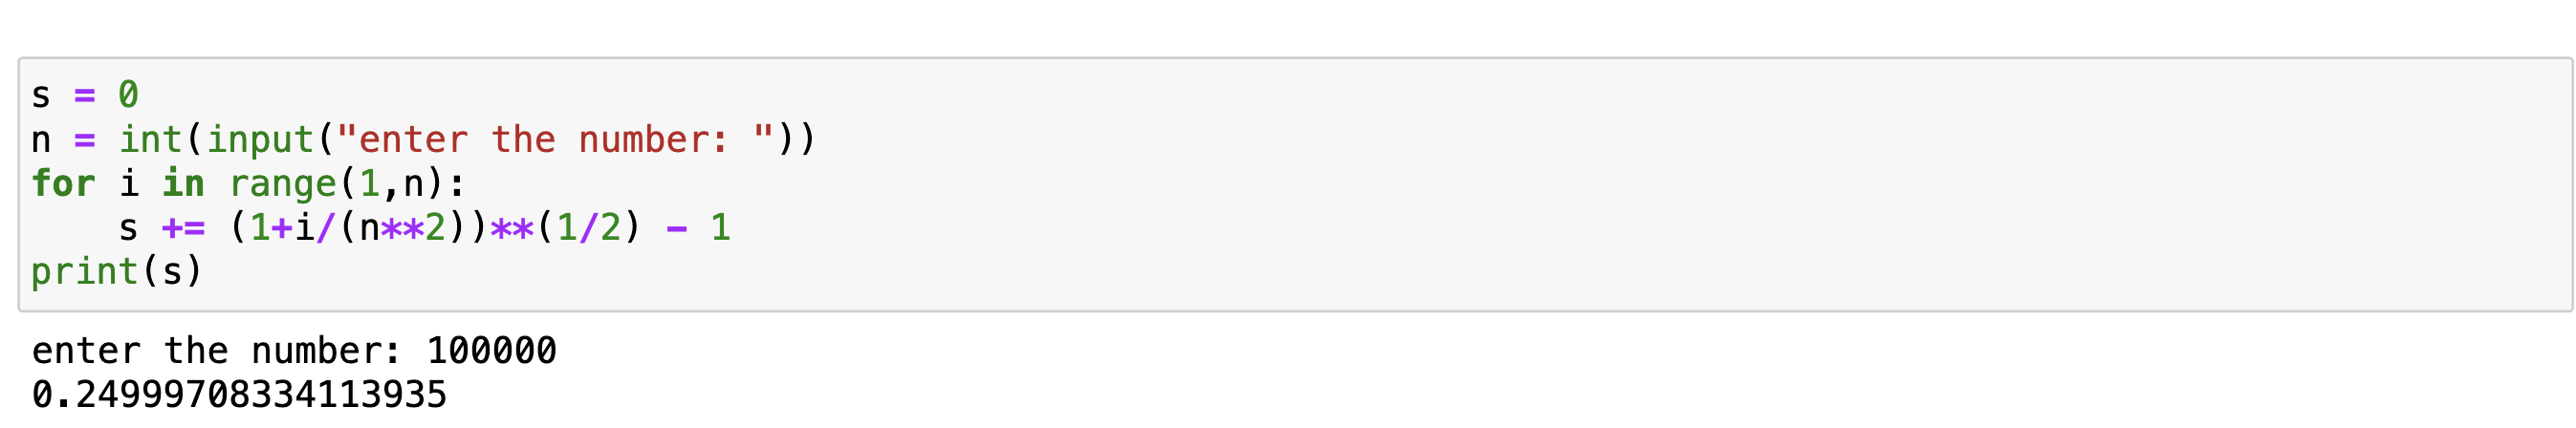
\includegraphics[scale = 0.35]{sequence in python.png}}
    \caption{This figure means that if we take n = 100000, $a_n \approx 0.2499970$}
    \label{fig}
\end{figure}
\\
\\
\\
\\
\\
\\
\tb{Q2} (Prime numbers with limit of sequence)\\
Denote the number of prime numbers which can divde $n$ as $p(n)$, prove that
$$
\lim_{n \to \infty} \frac{p(n)}{n} = 0
$$
\tb{Proof}: Now consider, if $p$ is a prime number who can divde $n$. Then there must exist one number $k$, 
such that $p \cdot k = n$. One can prove from this equality that one of them must be less than $\sqrt{n}$.
This implies that all the prime numbers who can divde $n$, they can be either less than $\sqrt{n}$ or the paired
number will be less than $\sqrt{n}$. So we split them into two cases, case one is that the prime number is less than
$\sqrt{n}$, those numbers can be at most $\sqrt{n}$. And for those prime numbers who are factors of $n$, we can count them 
by using the paired number of them, this can be at most $2\sqrt{n}$. So we can get two inequalities for $\frac{p(n)}{n}$, i.e.
$$
0< \frac{p(n)}{n} < \frac{2\sqrt{n}}{n}
$$
Again, we use sandwich theorem, $\lim_{n \to \infty} \frac{p(n)}{n} = 0$.\\
\\
\\
\\
\\
\\
\tb{Q3}\\
Let $a_0, a_1, \dots a_p$ be $p+1$ fixed numbers which satisfy 
$$
a_0 + a_1 + \dots + a_p = 0
$$
Find 
$$
\lim_{n \to \infty} (a_0 \sqrt{n} + a_1 \sqrt{n+1} + \dots + a_p \sqrt{n+p})
$$
\tb{Solution}: Notice that $a_0 = - a_1 - a_2 -\dots - a_p$, which helps us to simplify the equation into
$$
a_1 \cdot (\sqrt{n+1}-\sqrt{n}) + a_2 \cdot (\sqrt{n+2}-\sqrt{n}) + \dots + a_p \cdot (\sqrt{n+p}-\sqrt{n})
$$
Since those numbers are fixed and $p$ is just a constant, so we can deduce that
$$
\lim_{n \to \infty} (a_0 \sqrt{n} + a_1 \sqrt{n+1} + \dots + a_p \sqrt{n+p}) = 0
$$
Done!\\
\\
\\
\\
\\
\\
\tb{Q4} (Supremum and infimum)\\
Prove that for any sequences $\{x_n\}$ and $\{y_n\}$, following inequailties are true
\begin{center}
    $\sup\{x_n + y_n\} \leq \sup\{x_n\} + \sup\{y_n\}$\\
    $\inf\{x_n + y_n\} \geq \inf\{x_n\} + \inf\{y_n\}$
\end{center}
Pick one example where the strict inequailty holds, and pick an example that equality holds.\\ Prove also that 
if $A$ and $B$ are sets of numbers which are bounded above, then
$$
C \subset \{x+y\text{ }|\text{ }x\in A, y \in B\} \implies \sup C \leq \sup A + \sup B
$$
and
$$
\{x+y\text{ }|\text{ }x\in A, y \in B\} \subset C \implies \sup C \geq \sup A + \sup B
$$
Hence deduce that if $C = \{x+y\text{ }|\text{ }x\in A, y \in B\}$, then $\sup C = \sup A + \sup B$.\\
(I leave this as an exercise)\\
\\
\\
\\
\\
\\
\tb{Q5} (Bolzano-Weierstrass)\\
State Bolzano-Weierstrass theorem. Prove that a sequence has a convergent subsequence iff the sequence does not diverge to infinity. 
Use Bolzano-Weierstrass further deduce that a sequence is convergent iff it's a Cauchy sequence.
\newpage
\section{Day 6}
\subsection{Contraction mapping}
\tb{Q1} (Contraction mapping)\\
\tb{Definition}: Function $f$ is called a contraction mapping if $f$ is defined on $[a,b]$. $f([a,b])\subset [a,b]$ and there exists a constant $k$, 
such that $0<k<1$. And $\forall x,y \in [a,b]$, $|f(x)-f(y)| \leq k |x-y|$.\\
Prove the following statements:\\
1. $f$ has an unique invariant point $\xi$, i.e. a point which satisfies $\xi = f(\xi)$\\
2. For any initial value $a_0$, if the sequence is defined as $a_{n+1}=f(a_n)$, then this sequence must converge to $\xi$.\\
3. For every $a_n$,
$$
|a_n - \xi| \leq \frac{k}{1-k} |a_n - a_{n-1}| \text{ \ \ and \ \ } |a_n - \xi |\leq \frac{k^n}{1-k} |a_1-a_0|
$$
\tb{Proof}:\\
First I am going to prove that such $\xi$ exists for such function, which we can pick an arbitrary sequence $\{a_n\}$ with initial term $a_0$ within the domain of the function $f$.
Here I claim that this sequence is convergent. We can test this claim by proving it is a Cauchy sequence. Consider
\begin{align}
|a_{n+p}-a_{n}| = |f(a_{n+p-1}) - a_{n-1}| \leq k|a_{n+p-1}-a_{n-1}|
\end{align}
Then apply this procedure $n$ times, we obtain that
$$
|a_{n+p}-a_n| \leq k^n |a_{p}-a_0| \leq k^n |a-b|
$$
Since $k^n |a-b| \rightarrow 0$ as $n \rightarrow \infty$, one can always find an $N$, such that $\forall n \geq N$,
$|a_{N+p}- a_N| < \epsilon$. Hence, we proved that for any sequence with initial value within the domain $[a,b]$, it is convergent and now we can call this limit $\xi$.
We can actually prove that $f(a_n) \rightarrow f(\xi)$, this is just because $|f(a_n)-f(\xi)| \leq k|a_n - \xi|$. As a result, one can show that $\xi = f(\xi)$.\\
Let us prove that this $\xi$ is unique, suppose there is another invariant point which is called $\eta$. Since we want to prove they are unique, just consider the distance between them. 
Notice that 
$$
|\xi - \eta| = |f(\xi)- f(\eta)| \leq k|\xi -\eta| < |\xi - \eta|
$$
if $|\xi - \eta| \ne 0$, so the only way to make sense is $\xi = \eta$. Now we are done on 1 and 2.\\
For 3, we just apply our properties again, one can show that 
$$
|a_n - \xi| = |f(a_{n-1})-f(\xi)| \leq k|a_{n-1}-\xi| \leq k(|a_n - a_{n-1}| + |a_n-\xi|)
$$
rearrange of this inequality leads to $|a_n - \xi| \leq \frac{k}{1-k} |a_n - a_{n-1}|$. Use (1), we obtain second inequality we want to prove.\\
\\
\\
\\
\\
\\
\subsection{Some important properties about $e$}
\tb{Q2} (Formal definition of $e$)\\
Define $a_n = \left ( 1+ \frac{1}{n}\right )^n$ and $b_n = \left ( 1+ \frac{1}{n}\right )^{n+1}$. Prove that $a_n$ is simply increasing and $b_n$ is simply decreasing. Prove also that $a_n$ and $b_n$ are bounded. 
Hence deduce that both $a_n$ and $b_n$ are convergent to same limit, define this limit as $e$. Prove further that 
$$
e = \sum_{n=0}^{\infty} \frac{1}{n!}
$$
\tb{Proof}:\\
Notice that 
$$
a_n = \left ( 1 + \frac{1}{n}\right )^{n} \cdot 1 \leq \left( \frac{n+2}{n+1}\right)^{n+1} = a_{n+1}
$$
where we use the AM-GM inequality in "$\leq$". Again, one can see 
$$
\frac{1}{b_n} = \left( \frac{n}{n+1}\right)^{n+1} = \left( \frac{n}{n+1}\right)^{n+1} \cdot 1 \leq \left( \frac{n+1}{n+2}\right) ^{n+2} = \frac{1}{b_{n+1}}
$$
this implies that $b_{n+1} \leq b_n$, i.e. $\{b_n\}$ is a simply decreasing sequence. Then let's prove that $a_n$ and $b_n$ is bounded above and below, respectively. 
Notice 
\begin{align*}
a_n = \sum_{k = 0}^{n} \binom{n}{k} \cdot \left( \frac{1}{n} \right)^{n-k} &= \sum_{k = 0}^{n} \frac{1}{k!} \cdot \left(1 - \frac{1}{n}\right) \dots \left(1 - \frac{k-1}{n}\right) \\
    &\leq \sum_{k = 0}^{n} \frac{1}{k!}\\
    &=1 + 1 + \frac{1}{2!} + \dots + \frac{1}{n!}\\
    &\leq 1 + 1 + \frac{1}{1\times 2} + \frac{1}{2\times 3} +\dots + \frac{1}{(n-1)\times n}\\
    &= 1 + 1 + 1 - \frac{1}{n-1}\\
    &\leq 3
\end{align*}
So $a_n$ is bounded above by $3$. Obviously, $b_n$ is bounde below by $0$. And we can see that $\lim_{n \to \infty} a_n  = e = \lim_{n \to \infty} a_n \cdot \left(1+\frac{1}{n}\right)$, where the 
right hand side is just $b_n$.\\
Finally, let's prove that $e = \sum_{k=0}^{\infty} \frac{1}{k!}$. Let's define $s_n = \sum_{k=0}^{n} \frac{1}{k!}$, obviously, 
$s_n$ is simply increasing and bounded above.(One can easily check this) So we assume that $s_n \rightarrow s$ as $n \rightarrow \infty$. Since
$$
a_n = \sum_{k = 0}^{n} \frac{1}{k!} \cdot \left( 1 - \frac{1}{n}\right) \dots \left(1 - \frac{k-1}{n}\right) \leq s_n
$$
So we can deduce that $e \leq s$.
Additionally, if we fix $m$ as a constant, then 
$$
a_n \geq \sum_{k=0}^{m} \frac{1}{k!} \cdot \left( 1 - \frac{1}{n}\right) \dots \left(1 - \frac{k-1}{n}\right)
$$
take $n$ to $\infty$, one can see that $e \geq s_m$. Hence one can deduce that $e\geq s$. Combine those two inequalities, we can obtain that
$e = s$.\\
\\
\\
\\
\\
\\
\tb{Q3} (How fact is the convergence of $e$)\\
Define $\epsilon_n = e - (1 + 1+ \frac{1}{2!} + \dots + \frac{1}{n!})$. Use Stolz theorem to prove that 
$$
\lim_{n \to \infty} \epsilon_n \cdot (n+1)! = 1
$$
By considering $e = \sum_{k = 0}^{\infty} \frac{1}{k!}$, show that $$\frac{1}{(n+1)!}< \epsilon_n < \frac{1}{n\cdot n!}$$\\
\\
\\
\\
\\
\tb{Q4} (Euler constant $\gamma$)\\
Prove first that 
$$
\frac{1}{n+1} < \ln{\left(1 + \frac{1}{n}\right)} < \frac{1}{n}
$$
Use inequality above to prove that $\{c_n\}$ is convergent, given that $c_n = 1 + \frac{1}{2} + \dots + \frac{1}{n} - \ln n $. 
Normally, we call this limit $\lim_{n \to \infty} c_n = \gamma$ Euler constant. Hence, use $c_n$ to find the following limit, 
$$
\lim_{n \to \infty} \left( \frac{1}{n+1} + \frac{1}{n+2} + \dots + \frac{1}{2n}\right)
$$\\
\\
\\
\\
\\
\\
\tb{Q5} (Trigonometric and $e$ sequence)\\
Find 
$$
\lim_{n \to \infty} n \sin(2\pi n! e)
$$
Use Stolz theorem to find 
$$
\lim_{n \to \infty} \frac{\sum_{k=0}^{n}\ln \binom{n}{k}}{n^2}
$$
Deduce that the geometric mean of binomial coefficients $\rightarrow$ $\sqrt{e}$ as $n\rightarrow \infty$
\newpage 
\section{Day 7}
\tb{Q1} (A recursion sequence used in Kepler equation)\\
Kepler obtained the following equation
$$
x - q \sin x = a
$$
where $a$ is an arbitrary constant and $0< q <1$. This equation can not be rearranged in order to solve 
$x$. But there is a method which can approximate the solution by using a recursion sequence. This method 
is to use $a_{n+1} = q \sin a_n +a$, where it states that we can use arbitrary initial value for the sequence.
Prove that this is true. \\
\tb{Proof}: Define function $f(x)= q \sin x + a$, we want to apply contraction mapping theorem here. For any $x\in \mathbb{R}$, 
one can show that $f(x) \in [a-q,a+q]$. So we4 can just define the function on $[a-q, a+q]$. Notice that $f([a-q,a+q]) \subset [a-q,a+q]$.
And $\forall x, y \in [a-q,a+q]$, we have 
\begin{align*}
|f(x)-f(y)| &= |q(\sin x -\sin y)|\\
            &= \left|q \cdot 2 \cdot \cos \left( \frac{x+y}{2}\right) \cdot \sin \left(\frac{x-y}{2}\right)\right|\\
            &\leq \left|q \cdot \cos \left( \frac{x+y}{2}\right) \cdot |x-y|\right|
\end{align*}
here, $k$ can be chosed to be $q$. This implies that $f(x)$ is a contraction mapping, one can use the theorem we proved before to deduce that 
there exists unique $\xi$, such that $\xi = f(\xi)$, which is just the $x$ we want. Additionally, use the second criteria that we proved, one can 
showt that any sequence converges to this value. Done!\\
\\
\\
\\
\\
\subsection{Heine-Borel Theorem}
\tb{Q2} (Heine-Borel Theorem)\\
If $\{G_\al\}$ is an open cover of closed interval $[a,b]$, then there exists one finite subset 
$\{G_1,G_2,\dots, G_n\}$ such that it is a finite open cover of $[a,b]$.\\
\tb{Proof}: Now suppose $[a,b]$ has an open cover $\{G_\al\}$. Now define 
$$
A = \{x \geq a\text{ }| \text{ }[a,x]\text{ has a finite open cover}\}
$$
Since $\{G_\al\}$ is an open cover of $[a,b]$, so there must exist such an open set which can contain point 
$a$, this is finite open cover since only one open set is involved in covering $[a,a]$. One can separate this into 
two cases now, one is $A$ is not bounded above, and the other is that $A$ is bounded above. For the first case, 
we have a finite open cover for $[a, \infty]$, so if we use the same open cover for $[a,b]$, $[a,b]$ must be covered. 
For the second case, suppose $A$ is bounded by $\xi$. Now we want to prove that $\xi \geq b$, so the only case we need to 
consider is that $\xi < b$. Since $\xi \in [a,b]$, one can always find an open interval $G_i$ which can cover $\xi$. 
By adding $G_1$ into the open cover which can cover $[a,\xi]$, it is still a finite open cover, but it must cover some number 
which is greater than $\xi$. This leads to contradition.\\
\\
\\
\\
\\
\\
\tb{Q3} (Stronger Heine-Borel theorem)\\
Suppose $\{G_\al\}$ is an open cover of $[a,b]$. Prove that there exists a positive number $\delta > 0$, such that $\forall x',x'' \in [a,b]$, which satisfy
$|x' - x''|< \delta$, we can always find an element of $\{G_\al\}$ which contains $x'$ and $x''$.\\
\tb{Proof}: Apply Heine-Borel theorem here, one can find a finite subset of $\{G_\al\}$ which covers $[a,b]$, assume it is $\{G_1, G_2, \dots G_n\}$. Now 
for each of the $G_i$, we can find its two endpoints as $a_i,a_{i+1}$. Collecting all the endpoints of $G_1$ to $G_n$ and arrange them in order, which is 
$$
x_1 < x_2 < x_3 < \dots < x_{m}
$$
Take $\delta = \min\{x_2 - x_1, x_3 - x_2, \dots ,x_m - x_{m-1}\}$. Now I claim that this is the $\delta$ we want to find. Here are several cases. Case one is that 
$x'$ and $x''$ are both inside some interval $[x_i, x_{i+1}]$. Since $x_i$ and $x_{i+1}$ are both some endpoints of some open interval, such that there must exist 
some $x_j$ where $j < i$ such that $x'$ and $x''$ are contained in an open interval in the form of $(x_j,x_k)$, where $k \geq i+1$. The second case is that $x'$ and 
$x''$ are at different side of an endpoint $x_i$. Since $|x'-x''|<\delta$, so they must be contained in $(x_{i-1},x_{i+1})$. And since $x_i$ is endpoint of an 
open interval, so there must be another open set which can contain it, this is at least $(x_{i-1},x_{i+1})$. Done!\\
\\
\\
\\
\\
\\
\tb{Q4} (equivalent definitions of upper limit)\\
Prove first that every sequence must have at least one limit point. Prove also that 
$$
\uplim_{n \to \infty} x_n = \lim_{n \to \infty} \sup_{k\geq n} \{x_k\}
$$
\tb{Proof}:\\
The first statement is very easy as an exercise.\\
First, let us develop several notation to make the question simplified. Denote 
$$
b_n = \sup_{k\geq n} \{x_k\} = \sup \{x_n, x_{n+1}, \dots\}
$$
Hence the thing we want to prove becomes equivalent to $\lim\limits_{n \to \infty} b_n = \uplim\limits_{n \to \infty} x_n$.
Here, we have several things to discuss with, one is that $b_n$ might be infinity at some time for $n$.  Notice that $b_n \geq x_n$, so $b_n$ can only tend to 
$+\infty$. If $b_n$ is infinity at some time, this can actually implies $x_n$ is not bounded. Consider if $x_n$ is bounded above. Then every $b_n$ will be less 
than $M$, given that $M$ is the upper bound of $x_n$. Impossible for $b_n$ to be $+\infty$, so in this case $x_n$ must be not bounded above, and this implies that
$\uplim\limits_{n \to \infty} x_n = \lim\limits_{n \to \infty} \sup_{k\geq n} \{x_k\} = + \infty$.\\
The remaining cases are those $b_n$ are finite, $\forall n$. We have $b_{n+1} \leq b_n$, so $\{b_n\}$ is a decreasing sequence. Let $b = \lim\limits_{n \to \infty} b_n$.
To be rigorous, one need to prove that a decreasing sequence must have only one limit point, which is denoted by $b$. This is easy to see, we can talk about it in two 
cases. One is that the $b_n$ is bounded below, done. Another case is that $b_n$ is not bounded below, which means $b_n \rightarrow -\infty$, at this time, we define 
$b = -\infty$. Here, it becomes clear that there are two cases we need to give a insight. One is that $b = -\infty$, noticing $x_n \leq b_n$ will solve this problem as 
it tells us $x_n \rightarrow -\infty$ as $n \rightarrow \infty$.\\
Final case it that $b$ is a finite number. Claim: $b$ is a limit point of $\{x_n\}$. One can choose $\epsilon = 1,\frac{1}{2}, \frac{1}{3}, \dots$. In each case, we have 
$$
b \leq x_{k_i} \leq b_{k_{i}} < b + \frac{1}{i}
$$
$x_{k_n}\rightarrow b$, $b$ is a limit point of $\{x_n\}$. Suppose now $c$ is another limit point of $\{x_n\}$. $\{x_{n_k'}\}$ has limit of $c$. However consider $\{b_{n_k'}\}$
We have $x_{n_k'} \leq b_{n_k'}$. So $c\leq b$, this proves that $b$ is the upper limit of $\{x_n\}$.\\
\\
\\
\\
\\
\subsection{Definitions of limit of functions}
\tb{Q5} (Equivalent definition of limits of functions)\\
Prove that the following definitions are equivalent to the definition of the limit of function.
\begin{align}
    &\forall \epsilon > 0, \exists \delta > 0, \forall x \in O_\delta (a) - \{a\}, |f(x) - A| \leq \epsilon \tag{Definition 1}\\
    &\forall \epsilon > 0, \exists \delta > 0, \forall x \in O_\delta (a) - \{a\}, |f(x) - A| < k\epsilon \tag{Definition 2}\\
    &\forall n \in \mathbb{N}, \exists \delta > 0, \forall x \in O_\delta (a) - \{a\}, |f(x) - A| < \frac{1}{n} \tag{Definition 3}\\
    &\forall \epsilon > 0, \exists n, \forall x \in O_\frac{1}{n} (a) - \{a\}, |f(x) - A| < \epsilon \tag{Definition 4}
\end{align} 
(Leave as an exercise)
\newpage
\section{Day 8}
\subsection{Cantor set}
\tb{Q1} (Cantor set)\\
Denote $[0,1]$ as $E_0$. Now eliminate $\left(\frac{1}{3},\frac{2}{3}\right)$ from $E_0$ and denote the remaining closed interval as $E_1$. 
Show that 
$$
E_1 \supset E_2 \supset E_3 \dots
$$
Call $P = \bigcap_{n=1}^{\infty} E_n$. Prove that there is no open intervals of the form $\left( \frac{3k+1}{3^m}, \frac{3k+2}{3^m}\right)$ in $P$. Hence deduce 
that there is no open intervals contained in $P$.\\
\\
\\
\\
\\
\\
\tb{Q2}\\
Prove that for $0 < k < 1$, 
$$
\lim_{n \to \infty}[ (1+n)^k - n^k] = 0
$$
\tb{Proof}: Consider following inequality first,
$$
(1+n)^k - n^k = n^k \cdot \left(\frac{(1+n)^k}{n^k} - 1\right) = n^k \cdot \left(\left(\frac{1+n}{n}\right)^k - 1\right) \leq n^k \cdot \left( 1 + \frac{1}{n} - 1\right)
$$
By sandwich's theorem, we can see that 
$$
\lim_{n \to \infty} 0 \leq \lim_{n \to \infty} [ (1+n)^k - n^k] \leq \lim_{n \to \infty} n^{k-1} 
$$
And the left hand side and right hand side is both $0$, so we obtain the limit is $0$.\\
\\
\\
\\
\\
\\
\tb{Q3} \\
Suppose $\{x_n\}$ is convergent. Define 
$$
y_n = n(x_n - x_{n-1})
$$
Will $\{y_n\}$ be convergent?\\
\tb{Proof}: There are two ways of doing this, one is using an algebraic trick and another one is to prove it directly 
from definition. Let's do the \textcolor{blue}{tricky one}, $y_n = n(x_n - x_{n-1}) = nx_n -(n-1)x_{n-1}- x_{n-1}$. Then 
consider 
$$
\frac{y_1 + y_2 + \dots + y_n}{n} = \frac{nx_n - (x_1 + x_2 + \dots + x_{n-1})}{n}
$$
Now use Stolz, one can show that 
$$
\lim_{n \to \infty} y_n  = \lim_{n \to \infty} \frac{y_1 + y_2 + \dots + y_n}{n} = \lim_{n \to \infty}\frac{nx_n - (x_1 + x_2 + \dots + x_{n-1})}{n} = \lim_{n \to \infty} x_n - \lim_{n \to \infty} x_{n-1} = 0
$$
This implies that $\{y_n\}$ is not only convergent, but convergent to $0$.\\
\\
\\
\\
\\
\\
\tb{Q4} (Some properties about lower limit)\\
A finite number $b$ is the lower limit of $\{x_n\}$ iff \  $\forall \epsilon > 0$, there exists infinite terms of 
$\{x_n\}$ in $(b - \epsilon, b + \epsilon)$ and $\exists N$, $\forall n \geq N$, $x_n > b - \epsilon$.\\
\tb{Proof}:
Let do $\Longrightarrow$ first. Since $b$ is a limit of subsequence of $\{x_n\}$. Then there must exist infinite 
terms in $(b - \epsilon, b + \epsilon)$. Now we just want to show that $\exists N$, $\forall n \geq N$, $x_n > b - \epsilon$. 
Suppose $\forall N$, $\exists n \geq N$, such that $x_n \leq b - \epsilon$. We can do the following procedure, pick $N = 1$ first,
then we can find a $x_{n_1} \leq b - \epsilon$, taking $N = n_1+1$ now. There is always $x_{n_2}$, such that $x_{n_2} \leq b - \epsilon$.
Continue this procedure, one can show that there exists a sequence which has all the terms less than $b-\epsilon$. And this can imply that 
we must have a limit point less than $b$. Contradiction. Done!\\
Now let's do $\Longleftarrow$. $b$ is obviously a limit point of $\{x_n\}$, which we can verify this by considering $\epsilon = \frac{1}{n}$
at each time. The only thing left is to prove that this is the lowest limit point of this sequence. Now suppose there is $p < b$, where $p$ is 
a limit point of this sequence. So there must exist infinite terms between a small interval of $p$, this contradicts the second condition, since 
we can not find such a $N$ which satisfies $\forall n \geq N$, $x_n > b - \epsilon$. \\
\\
\\
\\
\\
\tb{Q5} (Why upper limits and lower limits are so useful)\\
Use upper-lower limits method to prove that a Cauchy sequence must be convergent. Use upper-lower limits to prove that a sequence defined as below is 
covergent.\\
Define $a_1 > 2$, and 
$$
a_{n+1} = 2 + \frac{1}{a_n} \text{ for } n \geq 1
$$
(this is from 2024 Jan analysis question)\\
\tb{Proof}: I leave this one as an exercise.\\
\newpage
\section{Day 9}
\subsection{General continuity for a polynomial}
\tb{Q1}\\
Prove that polynomials $p_n(x) = a_0 x^n +a_1 x^{n-1} + \dots + a_n$ is continuous at every point.\\
\tb{Proof}: This is equivalent to prove following:
$$
\lim_{x \to a} p_n(x) = p_n(a)
$$
We just need to prove that $\lim\limits_{x \to a}x^i =  a^i$, where $c$, $i$ are both constant. Then use the addition property of limit, 
one can then deduce what we want to prove. $\forall \epsilon > 0$, let's first take $\delta < 1$. Consider if $|x-a|< \delta$,
one can say that $|x|<|a|+ 1$, so now $|x|$ is bounded. Suppose it is bounded by $m$. Now take $M = \max\{|a|, m\}$. Let's then take $\delta < \frac{\epsilon}{iM^{i-1}}$.
Then we have the following inequailties:
$$
|x^i - a^i| = |x-a|\cdot|x^{i-1}+x^{i-2}\cdot a + \dots + a^{i-1}|\leq |x-a|\cdot(i \cdot M^{i-1})<\epsilon
$$
Notice that the final inequality is obtained by $\delta < \frac{\epsilon}{iM^{i-1}}$. Final thing to do is to apply the addition property and scalar multi property. Done!\\
\\
\\
\\
\\
\\
\subsection{Composition of limits}
\tb{Q2}\\
Given that $F(x) = f(g(x)) \text{, } \forall x$, with the conditions $\lim\limits_{x \to a}g(x) = A$ and $\lim\limits_{y \to A}f(y) = B$. Does this imply that 
$$
\lim_{x \to a}F(x) = \lim_{x \to a}f(g(x)) = \lim_{y \to A} f(y) = B\text{?} 
$$
\tb{Solution}: This is impossible, the following is a quick thought. For $f(g(x))$, if we want the limit of this one is same as $f(y)$, we need to restrict the 
$g(x)$ input to be different from $A$. However, we only have $g(x) \rightarrow A$, we do not have a condition to let $g(x)$ to be different from $A$. This might 
be like $g(x)$ is $A$ during small interval near $a$, and this would imply that the limit of $F(x)$ to be exactly the value at $A$ for $f(y)$.\\
After saying those, let's just pick one example when this is not true.
\begin{empheq}[left={f(y) =\empheqlbrace}]{align*}
    1 & \text{\ \ \ \  if } y \ne 0 \\
    0 & \text{\ \ \ \  if } y = 0
\end{empheq}
And $g(x) = 0$. So we notice that $\lim\limits_{x \to 0}f(g(x)) = 0$, but $\lim\limits_{y \to 0} f(y) = 1$. They are not equal.\\
\\
\\
\\
\\
\\
\tb{Q3} (Conditions which the composition of limits hold)\\
Suppose $\lim\limits_{x \to a}g(x) = A$, $\lim\limits_{y \to A}f(y) = B$. Then if one of the following conditions are satisfied,
\begin{align}
    &\exists B = (a-\delta_0, a+\delta_0)\setminus \{a\}\text{,\ \  } g(x) \ne A \text{ if } x \in B \tag{Condition 1}\\
    &\lim_{y \to A}f(y) = f(A)\tag{Condition 2}\\
    &A = \infty \text{ and } \lim_{y \to A}f(y) = B \tag{Condition 3}
\end{align}
Then 
$$
\lim_{x \to a} F(x) = \lim_{y \to A} f(y)
$$
(Leave this as an exercise)\\
\\
\\
\\
\\
\\
\\
\\
\\
\\
\\
\\
\\
\\
\tb{Q4} (Limited possibilities)\\
Prove that if $\lim\limits_{x \to a}g(x) = A$ and $\lim\limits_{y \to A}f(y)$, then $\lim\limits_{x \to a}f(g(x))$ only has three possibilities.\\
1. $\lim\limits_{x \to a}f(g(x)) = B$\\
2. $\lim\limits_{x \to a}f(g(x)) = f(A)$\\
3. the limit does not exist\\
(Also leave this as an exercise)\\
\\
\\
\\
\\
\\
\tb{Q5}\\
Prove that $\lim\limits_{x \to 0} f(x)$ exists iff $\lim\limits_{x \to 0}f(x^3)$ exists and they are equal when both exist.\\
\newpage
\section{Day 10}
\tb{Q1} (Limit only at one point)\\
Pick an example of a function where it is defined at $(-\infty, +\infty)$ with limit only at $x = 0$. That is, at any other point,
the function does not have a limit.\\
\tb{Solution}: Just consider the following function
\begin{empheq}[left={f(x) =\empheqlbrace}]{align*}
    x & \text{\ \ \ \  if $x$ is rational}  \\
    -x & \text{\ \ \ \  if $x$ is irrational}
\end{empheq}
Now, let's prove that it has limit at zero. $\forall \epsilon > 0$, just let $\delta = \epsilon$, notice that if $0<|x|<\delta$,
then $|f(x)- 0| = |x| < \epsilon$. Then the second thing we should do for this function is to prove it does not have limit at any 
other point. Suppose $x_0 \ne 0$, now let us take two sequences $\{a_n\}$ and $\{b_n\}$ both converges to $x_0$. But $a_n$ are all 
rational and $b_n$ are all irrational. We can see $f(a_n)$ tends to $x_0$, but $f(b_n)$ tends to $-x_0$.(We can carefully prove those
two properties). Now by Heine's theorem(we will prove later), this is impossible for $f(x)$ to have a limit at $x_0$.\\
\\
\\
\\
\\
\\
\tb{Q2} (Periodic function with its limit)\\
Prove that if $f$ is periodic function and $\lim\limits_{x \to \infty}f(x) = 0$, then $f(x)\equiv 0$.\\
\tb{Proof}: This one is an obvious one we should use contradiction to solve. Suppose $f(x_0) = a \ne 0$ for some $a$. Since $f$ is 
periodic, there will be $T > 0$ as its period. So $\forall N \in \mathbb{N}$, we have $f(x_0 + N T) = f(x_0) \ne 0$.\\ Let's prove the 
negation of $\lim\limits_{x \to \infty}f(x) = 0$. Set $\epsilon = |a|$, $\forall M > 0$, there must be $x_0 + N' T > M$, this follows 
from Archimedean property. So $\exists x = x_0 + N'T> M$, such that $|f(x)- 0| = |a|\geq \epsilon$. This means that we proved the 
negation of this statement.\\
\\
\\
\\
\\
\\
\tb{Q3} (Periodic rational functions)\\
Prove that all non-constant rational functions can not be periodic.\\
(Leave as an exercise)\\
\\
\\
\\
\\
\\
\tb{Q4} (One-sided limit for functions)\\
Suppose $a$ is a finite number, then 
$$
\lim_{x \to a} f(x) = A
$$
if and only if $f(a^{-}) = f(a^{+}) = A$. A can either be finite or infinite.\\
\tb{Proof}: ($\Longleftarrow$) By definitions of one-sided limit, $\forall \epsilon > 0$, we can always find $\delta_1$ and $\delta_2$, such that, 
$\forall x \in a-\delta_1 < x < a \text{ and } a< x < a + \delta_2$, $|f(x) - A| < \epsilon$. We then take $\delta = \min\{\delta_1, \delta_2\}$,
for $0< |x -a |< \delta$, we have $|f(x) - A|< \epsilon$.\\
($\Longrightarrow$) $\forall \epsilon > 0$, $\exists \delta > 0$, $\forall x \in 0 < |x - a| < \delta$, $|f(x) - A| < \epsilon$. Now for each side,
just take $\delta_1 = \delta_2 = \delta$, this works to show that both sides tends to $A$. Done!\\
\\
\\
\\
\\
\\
\tb{Q5}\\
Suppose $f$ is monotone on $(a,b)$, then $f(b^{-}) = \lim\limits_{x \to b^{-}} f(x)$ must be meaningful.\\
\tb{Proof}: Wlog, let's assume that $f(x)$ is increasing on $(a,b)$. Now, let $A = \{a\text{ }|\text{ }\exists x \in (a,b), f(x) = a \}$. Since $(a,b)$
is not empty, so we can say that $A$ is not empty, it must have a $\sup A$ if finite. Now we are dealing with two cases. Case one is that $A$ is bounded 
above. In this case, let $\xi = \sup A$. Using the property of supremum, $\forall \epsilon > 0$, there must exist one $x' \in A$, such that $f(x') > \xi -\epsilon$ 
and then we claim that $\forall x \in A > x'$, we have $\xi - \epsilon< f(x') \leq f(x) \leq \xi$. This actually implies that $\lim\limits_{x \to b^{-}} f(x)$.\\
Then the case left is when $A$ is not bounded. Now we claim that $\lim\limits_{x \to b^{-}} f(x) = + \infty$. This is because $\forall M > 0$, there must be $x \in (a,b )$,
such that $f(x) > M$, take $b-x$ as $\delta$, one can show from the definition that $\lim\limits_{x \to b^{-}} f(x) = +\infty$. Done!\\
\newpage
\section{Day 11}
\subsection{Alternative definition of closed sets}
\tb{Q1}\\
Show that a set $B$ is closed if and only if $\forall \text{ convergent }\{x_n\}\subset B$, where
$$
\lim_{n \to \infty}x_n = x
$$
we have $x \in B$.\\
\tb{Proof}:\\
($\Longrightarrow$) $B$ is closed, $B^c$ is open. We can actually show that $\forall b \in B^c$, it can not be the limit of any convergent sequence in $B$. There exists $\delta$, 
such that $(b-\delta, b+\delta) \subset B^c$. Hence if one sequence tends to $b$, we can let $\epsilon = \delta$, this would result in there must be infinite terms of $\{x_n\}$ in 
$B^c$. Contradiction, so we must have all limit of convergent sequences in $B$ to be one element in $B$.\\
($\Longleftarrow$) Suppose $B^c$ is not an open interval, so exists $b \in B^c$, such that $\forall \epsilon > 0$, $\exists b' \in B$, such that $b' \in (b-\epsilon, b+ \epsilon)$. Now 
take $\epsilon = \frac{1}{n}$ each time, so we can find a sequence that is belong to $B$ but it tends to $b$. So we must have $b \in B$. Contradiction.\\
\\
\\
\\
\\
\\
\tb{Q2} (Referenced from Rudin)\\
\tb{Defintion} (Limit points)\\
A point $p$ is said to be limit point of set $E$, if $\forall \delta > 0$, $\exists q \in E$, such that, $q \ne p$ and $q \in N_\delta(p)$.\\
This is how we define a limit point on a metric space. Now go back to $\mathbb{R}$ for a moment.\\
Prove that $E$ is closed if and only if every limit point $p$ of $E$ belongs to $E$.\\
(Leave as an exercise)\\
\\
\\
\\
\\
\\
\subsection{Compact \& Closed and Bounded}
\tb{Q3}\\
\tb{Definition} (Compact sets)\\
A set $K \subset \mathbb{R}$ is compact if and only if every sequence $\{x_n\} \subset K$ contains a convergent subsequence $\{x_{n_i}\}$ and $\lim\limits_{i \to \infty} x_{n_i} \in K$.\\
Now prove that 
$$
K \text{ is compact} \Leftrightarrow K \text{ is closed and bounded}
$$
\tb{Proof}:\\
($\Longrightarrow$) Let's use Q1 in this direction. Since $\forall \text{  convergent } \{x_n\} \subset K$. $K$ is compact tells us that there is a subsequence converges to $k \in K$. From 
the property of connvergent sequences we know that $\{x_n\}$ must have same limit as its subsequence. So, $\{x_n\} \rightarrow k \in K$. Done!\\
($\Longleftarrow$) This side is very easy as we can use the Bolzano-Weierstrass theorem here to say that since the sequence is bounded, so it must have a subsequence which converges to some 
value in this $K$. Done!\\
\\
\\
\\
\\
\\
\tb{Q4} (Intervals that are compact)\\
Prove that intervals in the form of $\left[a , b\right]$ are compact. Then prove that all closed subsets of a compact set is compact.\\
\tb{Proof}:\\
Notice first that $\left[a, b\right]$ is closed and bounded, so it is compact. The second one is just some deductions of definitions. Let's call $A$ as any closed subset of $E$, where $E$ is the
compact set. Suppose $\{x_n\} \subset A$. $\{x_n\} \subset K$, there exists $\{x_{n_i}\}$ converges to some value $k \in K$. We can actually argue that $k \in A$. Then the question is done!\\
\\
\\
\\
\\
\\
\subsection{Equivalent definitions for Compact sets}
\tb{Q5}\\
Prove that a set $E$ is compact if and only if for every open cover of $E$, there will be a finite subsets $\{G_\alpha\}$ of open cover, such that
$$
E \subset G_{\al_1} \cup G_{\al_2} \cup \cdots \cup G_{\al_n}
$$ 
\tb{Proof}: Let's denote the finite open cover property as $P_F$. A set satisfies this property is called $P_F$ set. \\
($\Longrightarrow$) I will first prove that if a set is compact, then it must have property $P_F$. We proved before that if a set $E$ is compact, then it 
must be closed and bounded. Therefore, there must exist one $[a, b]$, containing $E$. Then I will introduce a \tb{theorem} first. \\
\tb{Theorem}: A closed subset of $P_F$ set must also be $P_F$ set.\\
Denote the $P_F$ set as $K$ and the closed subset of it as $E$. Let $\{V_\al\}$ to be any open cover of $E$. Now add $E^c$ into the $\{V_\al\}$. This means that the new open cover $\{U_\al\} = E^c \cup \{V_\al\}$
must be an open cover of $K$. Because $K$ is a $P_F$ set, then there must exist finite subset of $\{U_\al\}$ that can cover $K$. There are two cases remaining, one is that $E^c$ is in this set. If this is true, 
then take out $E^c$ from this subset, the remaining sets are a finite subset of $\{V_\al\}$ which also covers $E$. Another case is that $E^c$ is not in the subset, this finite subset of $\{U_\al\}$ is also a finite 
subset of $\{V_\al\}$, hence this can cover $E$. Done!\\
Let's come back to our proof now, using Heine-Borel's theorem we stated in \tb{Day 7}, one can show that $[a,b]$ is a $P_F$ set. Then $E$ must be a $P_F$ set.\\
($\Longleftarrow$) Let's then prove that if $E$ is a $P_F$ set, then $E$ is compact. Let's first prove that every infinite subset $K$ of $E$ must have a limit point $p \in E$. This can be done using contradiction. Suppose 
that there is no limit points of $K$ in $E$. Hence $\forall q \in E$, we can always find $\delta_q > 0 $, such that the open interval $(q - \delta_q, q + \delta_q)$ can contain at most $1$ point of $K$. So take all such 
open interval for all points in $E$. This is an open cover of $E$. However, there can not be finite subset of it which can cover $E$ since $K$ is infinite. This contradicts, so every infinite subset of $E$ must have a limit 
point in $E$. Then I am going to use this property to prove $E$ is bounded and closed. Suppose $E$ is not bounded, i.e. $\forall N \in \mathbb{N}$, we can find $|x_n| > N$ and $x_n \in E$. Now $\{x_n\}$ is an infinite subset of 
$E$, however it does not have any limit point in $\mathbb{R}$. So it does not have any limit point in $E$. Contradiction shows that $E$ must be bounded. Suppose $E$ is not closed, meaning that $\exists p \not \in E$, such that 
$p$ is a limit point of $E$ (Notice that this comes out directly from the alternating definition of closed set). If each time I take $\delta = \frac{1}{n}$, I can find $\{y_n\}$ such that $y_n \in E$ and $y_n \in (
p - \frac{1}{n}, p + \frac{1}{n})$. Since $\{y_n\}$ is an infinite subset of $E$, so it must have a limit point $y \in E$. However, the definition shows that the sequence must converge to only one limit, which is $p$.(One can show this
by contradiction). After proving this by oneself, we have proved that $E$ is bounded and closed, which is equivalent as $E$ being compact. Done!
\newpage
\section{Several ways of proving Bolzano Theorem}
\subsection{Bolzano Theorem}
Bolzano's theorem states that if $f$ is continuous on $[a,b]$ and assume 
$$
f(a) < 0 < f(b)
$$
then there exists $x \in (a, b)$, such that $f(x) = 0$. \\
This is an important theorem in continuity of a function, and there are a lot of ways to prove the theorem, which we will introduce later.\\
\\
\\
\\
\\
\\
\subsection*{Lebesgue method}
Let's use my favourite method to prove \tb{Bolzano Theorem} first. Notice that since $f(a)$ is less than zero and $f$ is continuous on $[a,b]$,
$\exists \delta > 0$, $\forall x \in [a, a + \delta)$, $f(x) < 0$. Now let's apply Lebesgue method here, define $A = \{x\text{ }|\text{ }x \in [a,b],\text{ }f(x) < 0\}$.
We notice that $A$ is non-empty and $A$ is bounded above. So we can apply the supremum theorem to $A$, let $\alpha = \sup A$. And now we have several things to do, first of 
all, we notice that $\alpha < b$ this is because there also exists an interval on the left of $b$, such that $f(x) > 0$ in this interval. So we can pick any 
element in this interval, one can show that $\alpha$ is less than this element, and this element is less than $b$. There are three possibilities there for $\alpha$.
$f(\alpha) > 0$, $f(\alpha) < 0$ and $f(\alpha ) = 0$. We only need to show that the first two possibilities can not happen here. Let's assume $f(\alpha) < 0$. Now since $f$ 
is continuous at $\alpha$, so we can find an element $\alpha' > \alpha$ and $f(\alpha' )< 0$, this contradicts that $\alpha$ is the supremum of $A$. Suppose now $f(\alpha) > 0$,
then there exists a small interval on the left of $\alpha$, for all $x$ in this interval, $f(x) > 0$. However, we can use property of supremum to contradict this. Done!
\\
\\
\\
\\
\\
\\
\subsection{Nested Intervals method}
Consider bisection of the interval of $[a,b]$. The first step is to consider $\frac{a+b}{2}$ and we test whether $f(\frac{a+b}{2})$ is less than zero or larger than zero. If $f(\frac{a+b}{2}) = 0$.
we proved the theorem. If $f(\frac{a+b}{2}) < 0$, let $a_1 = \frac{a+b}{2}$ and $b_1 = b$, similar for $f(\frac{a+b}{2}) > 0$. Constructing those $a_n$ and $b_n$. We have $|a_n - b_n| \leq \frac{|a-b|}{2^n}$,
by nested intervals theorem, $\exists \xi$ such that $\lim\limits_{n \to \infty}a_n = \lim\limits_{n \to \infty} b_n = \xi$. Then we can claim that $f(\xi) = 0$. If $f(\xi) \ne 0$, wlog, I assume that $f(\xi) > 0$. 
By continuity of $f$, we can prove that there exists a small interval of $\xi$, where all $f(x)$ in this interval remains the same sign as $f(\xi)$. However, this is impossible because we can always find $a_k$ 
in this interval such that $f(a_k) > 0$. Done!
\\
\\
\\
\\
\\
\subsection{Heine Borel method}
This method uses Stronger Heine Borel Thoerem in order to prove the statement. $f$ is continuous on $[a,b]$ suppose that we can not find a point $\xi \in (a,b)$, such 
that $f(\xi) = 0$. This implies that for all the value between $[a,b]$ , we can always find a small open interval which all the $f(x)$ inside it preserves the same sign 
as the point, so this forms an open cover of the interval $[a,b]$, apply stronger Heine Borel Theorem here, we see that there exists a $\delta$, which satisfies that 
$\forall x', x'' \in [a,b]$, if $|x' - x''| < \delta$, there exists an open interval from the set which can cover the points $x'$ and $x''$. Now we can further 
claim that $f(x')$ and $f(x'')$ have the same sign since they are contained in same open interval we constructed earlier. Now consider we divide the interval $[a,b]$ into some
pieces where each piece has a length of $\frac{\delta}{2}$, this implies that $f(a)$ has the same sign as $f(b)$, because that $f(a+\frac{\delta}{2})$ preserves the same sign as 
$f(a)$ which preserves the same sign as $f(a + \delta)$, continuing this process. This one is a contradiction, so we can now prove by contradiction 
that the bolzano theorem holds in this situation.\\
\newpage
\section{Day 12}
\tb{Q1}\\
Suppse $f$ is continuous on $[a,b]$, $\forall \text{ rational numbers }r_1, r_2 \in [a,b]$, $r_1 < r_2 \implies f(r_1) \leq f(r_2)$. Prove that $f$ is monotone increasing on $[a,b]$.\\
\tb{Proof}:\\
Prove by contradiction, assume that there exists two points $x_0$ and $x_1$ such that $x_1 < x_0$ but $f(x_1) < f(x_0)$ (This is the negation of montone increasing). Since $f$ is 
continuous, we can find $\delta_1$ and $\delta_0$ such that $\forall x \in (x_1 - \delta_1)$, $f(x)$ is greater than all $f(y)$ for $y \in  (x_0, x_0 + \delta_0)$. To be more specific, 
we can let $\delta_0 + \delta_1 < |x_1 - x_0|$. Pick any rational number in those two intervals, we can show a contradiction to the condition.\\
\\
\\
\\
\\
\\
\tb{Q2}\\
Prove that the discontinuities of monotone functions can only be jump points.\\
\tb{Hint}: Let's conside $f(x_0^-)$ and $f(x_0^+)$. Since the function is monotone, we can claim that those two limits exist and have an inequality 
$$
f(x_0^-) \leq f(x_0) \leq f(x_0 ^ +)
$$
However, it is discontinous at $x_0$, so one can actually show that the inequality should be strict, this is the definition of a jump point. Done!


\end{document}